%%%%%%%%%%%%%%%%%%%%%%%%%%%%%%%%%%%%%%%%%%%%%%%%%%%%%%%%%%%%%%%%%%%%%%%%
\chapter{The Memory System}
\label{sec:memory}
%%%%%%%%%%%%%%%%%%%%%%%%%%%%%%%%%%%%%%%%%%%%%%%%%%%%%%%%%%%%%%%%%%%%%%%%
In this section \SIM memory system is explained. First, we describe caches,
then memory system hierarchy and organization. Next, configuring different
memory systems are investigated. Finally, DRAM module is explained.

%%%%%%%%%%%%%%%%%%%%%%%%%%%%%%%%%%%%%%%%%%%%%%%%%%%%%%%%%%%%%%%%%%%%%%%%
\section{Caches}
%%%%%%%%%%%%%%%%%%%%%%%%%%%%%%%%%%%%%%%%%%%%%%%%%%%%%%%%%%%%%%%%%%%%%%%%

Each cache structure consists of the cache storage (tag and data) and multiple
queues. Figure~\ref{fig:cache} shows the overall structure and its queues
of a cache in \SIM. There are two flows to the cache:
\begin{enumerate}
 \item \textbf{Cache access flow}: from a processor or upper level cache
		\footnote{Due to miss in that level} to access the cache
 \item \textbf{Cache fill flow}: in case of a cache miss, data is supplied from the 
		lower level cache or DRAM.
\end{enumerate}
Section~\ref{sec:queue} details all queues and Section~\ref{sec:cache-flow}
lists the flows through the queues and the cache.

\begin{figure*}[htb]
  \centering
  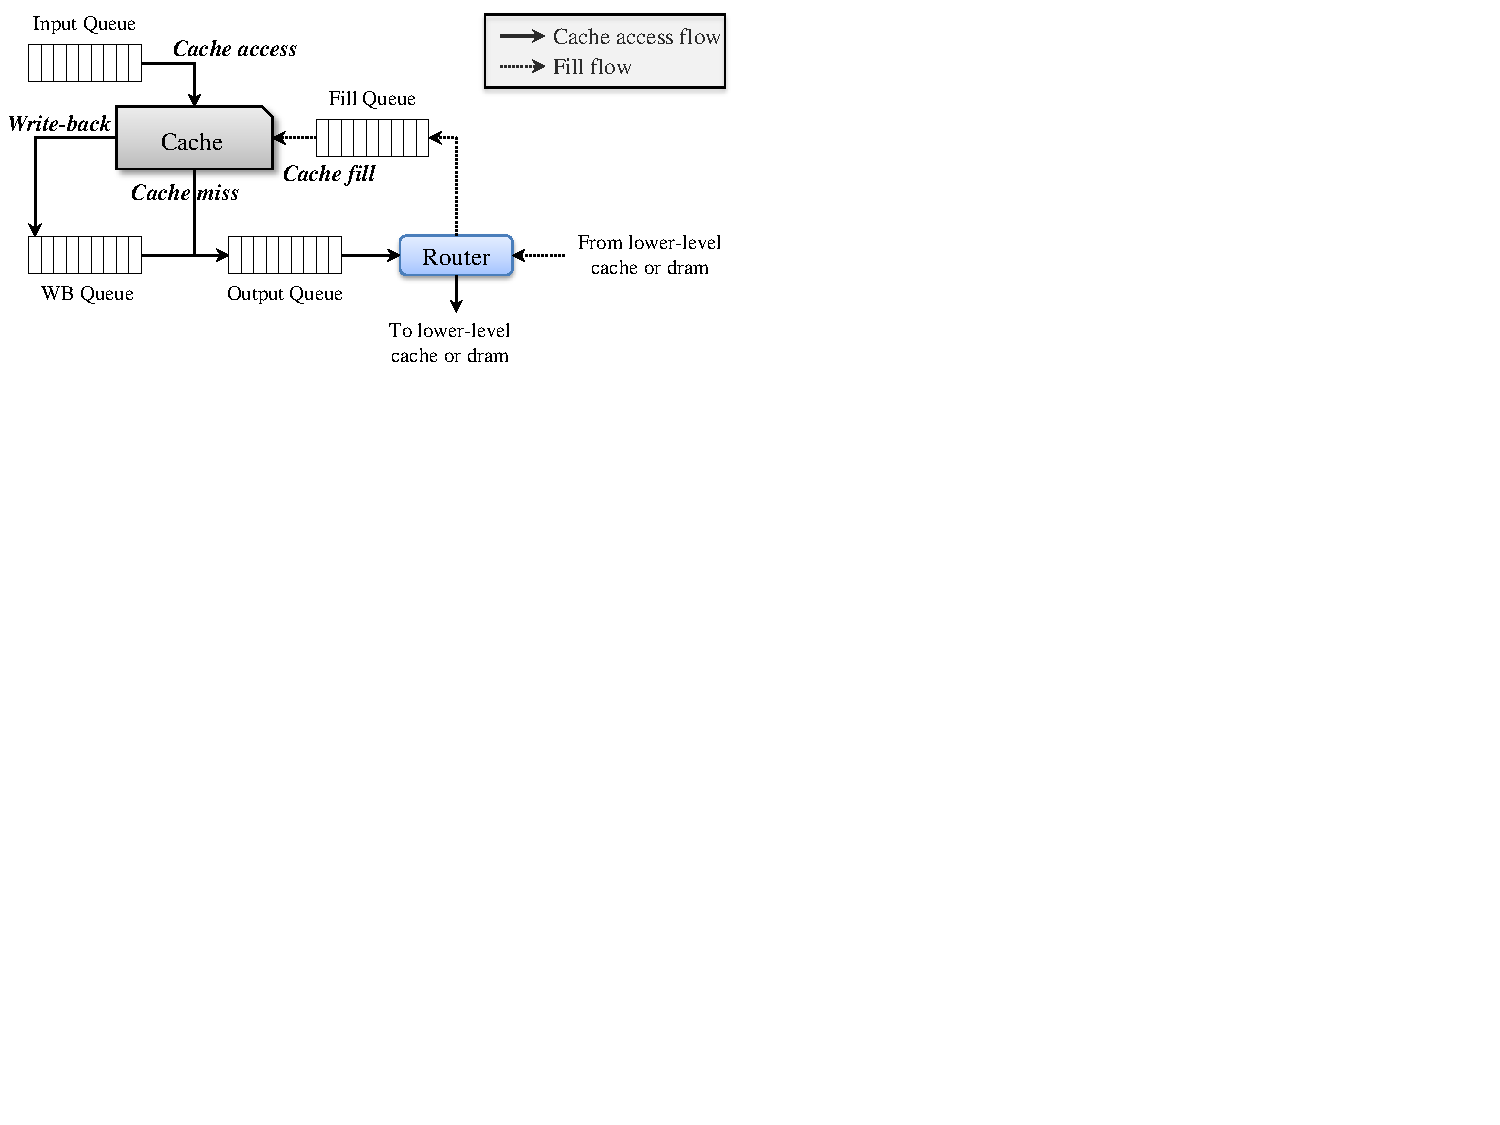
\includegraphics{figs/cache}
  \caption{The cache structure.}
  \label{fig:cache}
\end{figure*}

%%%%%%%%%%%%%%%%%%%%%%%%%%%%%%%%%%%%%%%%%%%%%%%%%%%%%%%%%%%%%%%%%%%%%%%%
\subsection{The Queues}
\label{sec:queue}
%%%%%%%%%%%%%%%%%%%%%%%%%%%%%%%%%%%%%%%%%%%%%%%%%%%%%%%%%%%%%%%%%%%%%%%%

\SIM uses queues to transfer data and command between different cache levels
and processors. Therefore, all cache accesses flow from one queue to another.
Below is the list of queues and their description.

\begin{itemize}
  \item \textbf{Input queue}: requests forwarded to the cache due to upper-level 
		cache misses or processor are inserted into this queue.

  \item \textbf{Output queue}: requests that miss in the cache are inserted into the
  output queue to be forwarded to a lower-level cache. If no lower-level cache
  is available, then requests are forwarded to the memory controller.

  \item \textbf{Write-back queue}: \SIM models write-back caches. When a dirty cache
  line is evicted, the line must be written back into the next level cache (or
  main memory). All write-back requests are initially inserted into this queue.

  \item \textbf{Fill queue}: Data returned from the next level cache or main memory 
  is inserted into the fill queue before updating the cache to be processed.

%  \item coherence queue - this queue is intended for handling coherence
%  traffic, but this is currently not modeled
  
\end{itemize}

%%%%%%%%%%%%%%%%%%%%%%%%%%%%%%%%%%%%%%%%%%%%%%%%%%%%%%%%%%%%%%%%%%%%%%%%
\subsection{The Flows}
\label{sec:cache-flow}
%%%%%%%%%%%%%%%%%%%%%%%%%%%%%%%%%%%%%%%%%%%%%%%%%%%%%%%%%%%%%%%%%%%%%%%%
In this subsection all possible flows from or to the cache is listed. If the memory or cache
levels are distributed, \SIM will use routers to send core's request. 

\begin{itemize}

  \item \textbf{Upper-level cache $\rightarrow$ Input queue}: Forwarding of upper-level cache misses
		to the cache.

  \item \textbf{Upper-level cache $\rightarrow$ Fill queue}: Forwarding of upper-level write-back 
		requests to the cache.

  \item \textbf{Input queue $\rightarrow$ Cache}: Accessing the cache

  \item \textbf{Cache $\rightarrow$ Output queue} : Cache miss, access to lower-level cache

  \item \textbf{Cache $\rightarrow$ Write-back queue}: Generating write-back requests due to
		eviction of a dirty line

  \item \textbf{Write-back queue $\rightarrow$ Output queue} : write-back requests to access the
		lower-level cache when they are processed.

  \item \textbf{Output queue $\rightarrow$ Router} : access the lower-level cache
		through the on-chip interconnection network

  \item \textbf{Router $\rightarrow$ Fill queue} : the data from the lower-level cache
		or DRAM

\end{itemize}

%%%%%%%%%%%%%%%%%%%%%%%%%%%%%%%%%%%%%%%%%%%%%%%%%%%%%%%%%%%%%%%%%%%%%%%%
\section{The Hierarchy}
\label{sec:memhierarchy}
%%%%%%%%%%%%%%%%%%%%%%%%%%%%%%%%%%%%%%%%%%%%%%%%%%%%%%%%%%%%%%%%%%%%%%%%

\SIM is very flexible in its support for different memory
hierarchies. Each level in the cache hierarchy can be configured
independently of other levels (see Section~\ref{sec:knob:cache}).
Figure~\ref{fig:memory} shows the base memory hierarchy without DRAM
memory. It is good to note these points about this figure: 

\begin{figure*}[htb]
\centering
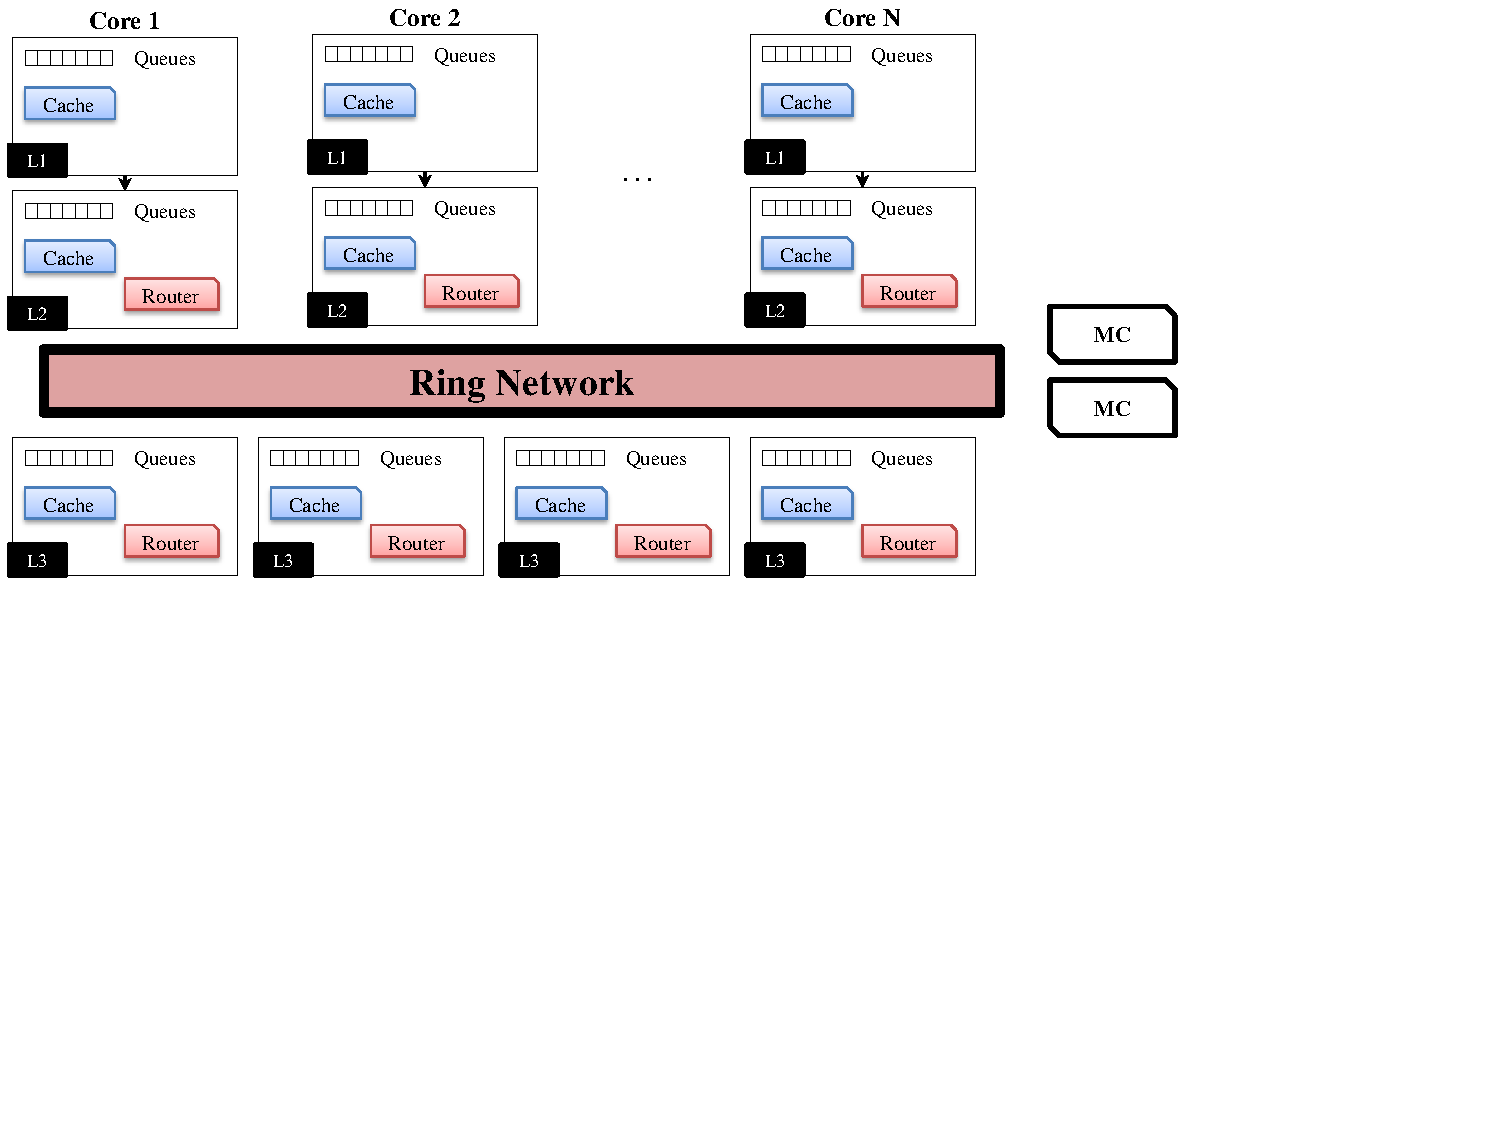
\includegraphics[width=6.5in]{figs/memory}
\caption{The memory system in \SIM.}
\label{fig:memory}
\end{figure*}


\begin{itemize} 
  \item There are three levels (L1, L2, and LLC) of caches in the
	\SIM , the L2 cache can be disabled if needed.

  \item All the caches and memory controllers can be connected via an
    on-chip interconnection network (currently, the default topology
    is ring), if the configuration allows.

  \item L1 and L2 caches are always private to each core.

  \item The local router within a cache structure is enabled only when
	necessary.

  \item LLC cache is unified (shared by all cores), but sub banked. In
    other words, address regions are statically partitioned and each
    tile is responsible for sub regions. Each cache tile has multiple
    banks as well.
   
  \item Each LLC tile could be coupled with its own L2 to reduce network
	  traffic. This is controlled by knob \Verb+memory_type   llc_[de]coupled_network+.
	  For more setting for this knob look at \ref{sec:types_memory}.

\end{itemize}


Figure~\ref{fig:level2cache} shows how to configure a 2-level cache hierarchy.
Even though there are 3-levels of cache, the L2 cache is disabled and only its
router is used by the L1 cache to access the interconnection network. Since
there is no additional latency between L1 and L2 when the L2 is disabled, we
can flexibly configure 2-level cache hierarchies.


\begin{figure*}[htb]
\centering
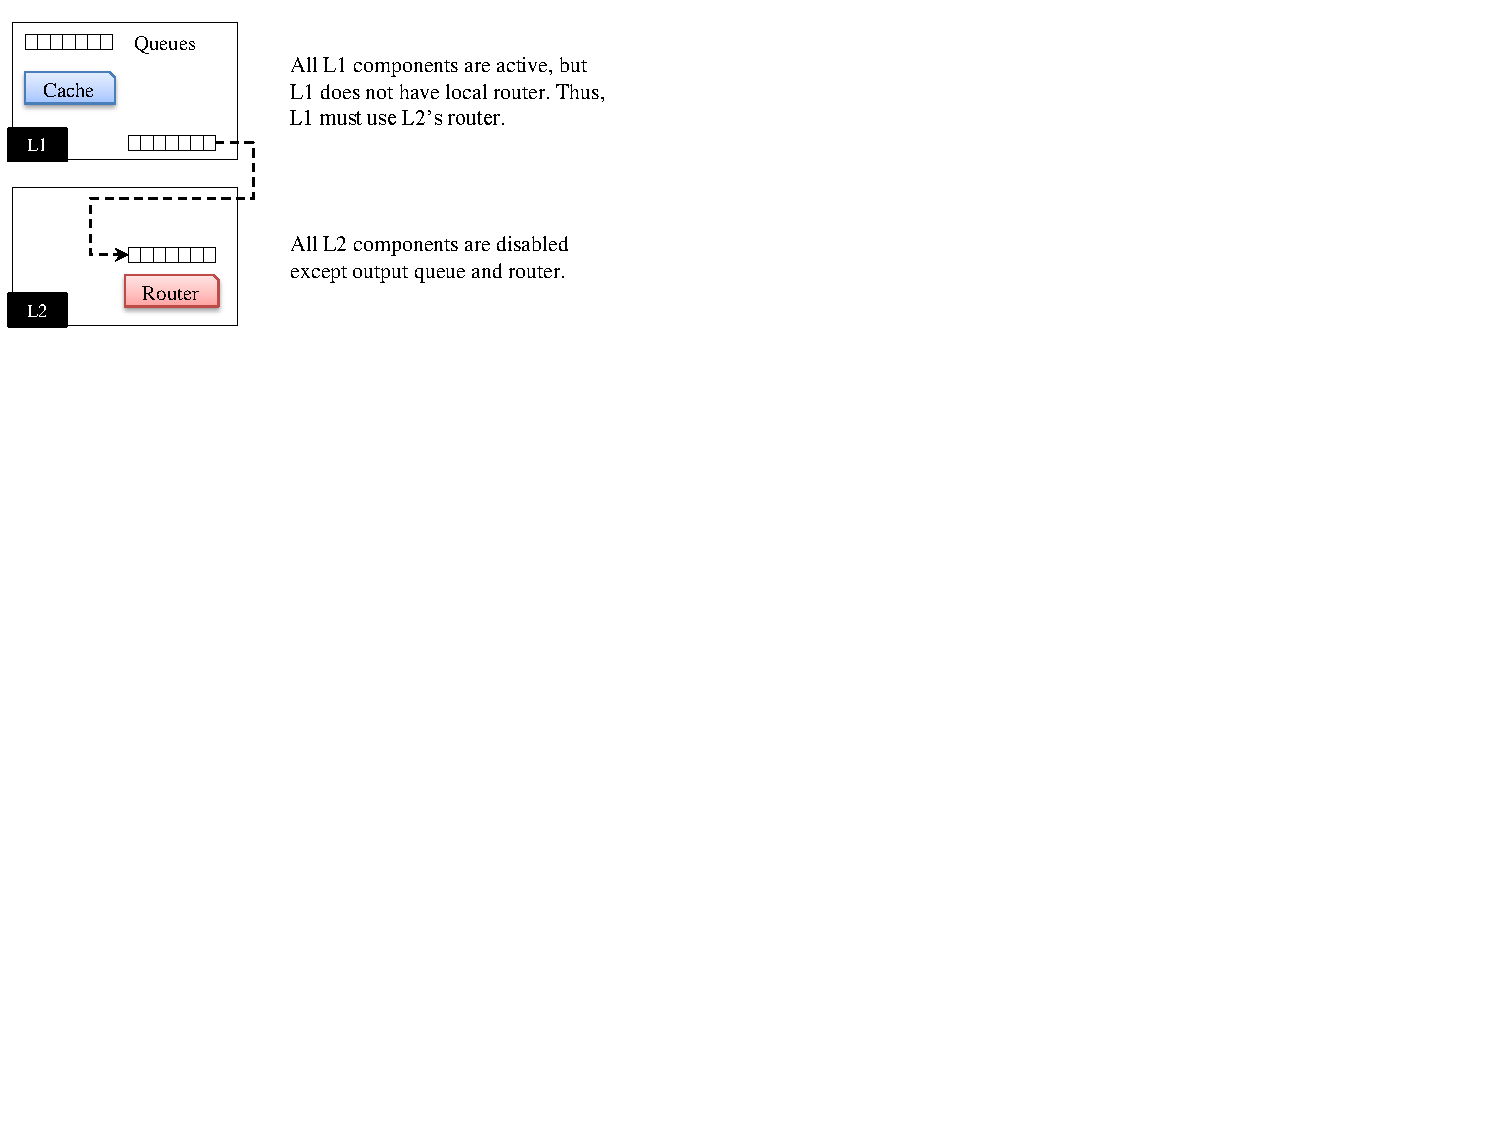
\includegraphics{figs/level2cache}
\caption{2-Level cache hierarchy.}
\label{fig:level2cache}
\end{figure*}

%%%%%%%%%%%%%%%%%%%%%%%%%%%%%%%%%%%%%%%%%%%%%%%%%%%%%%%%%%%%%%%%%%%%%%%%
\section{Configuring the Cache Hierarchy} 
%%%%%%%%%%%%%%%%%%%%%%%%%%%%%%%%%%%%%%%%%%%%%%%%%%%%%%%%%%%%%%%%%%%%%%%%

The cache hierarchy can be configured by:
\begin{enumerate}
 \item Setting the links between different cache levels
 \item Disabling cache levels
 \item Enabling/Disabling routers
\end{enumerate}
Following variables is used in \SIM for cache initialization:

\begin{center}
\begin{tabular}{l | l}
  Variable Name & Description \\ \hline \hline
  int next\_id & next level cache id \\
  int prev\_id & previous level cache id \\ 
  bool coupled\_up &  direct link with upper level cache \\
  bool coupled\_down & direct link with lower level cache \\
  bool disable & disable cache \\
  bool has\_router & router \\ 
\end{tabular}
\end{center}

\begin{description}
  \item[Enabling/disabling router] When \textsf{has\_router} is set to \textit{false},
  the cache cannot directly access to the on-chip
  interconnection. Instead, it has to go through lower-level cache's
  interface. Therefore, \textsf{coupled\_down} must set
  to \textit{true} and appropriate \textsf{next\_id} must be set. In
  this way, the output queue of the cache is connected directly to the
  input queue of the next level (lower) cache.

  \item[Disabling cache levels] When \textsf{disable} is set to \textit{true},
  the cache is disabled. When a request is inserted into the input queue of a
  disabled cache, the request will be directly inserted into the output queue
  of the cache. This feature has been used for modeling 2-level cache
  hierarchies. As Figure~\ref{fig:level2cache} shows, L1 and LLC caches are
  active, but L2 cache is disabled. However, since the L1 cache does not have a
  router, it needs to use the router of the L2 cache. Therefore,
  \textsf{has\_router} must be set to \textit{true} for the L2 cache.

  \item[Links] As mentioned in the Section~\ref{sec:memhierarchy}, the
  L1 and L2 caches are always private to a core. All L1 misses
  should go through the L2 cache without accessing the interconnection
  network. To this end, a direct link must be set between the L1 and
  L2 caches. Therefore, \textsf{coupled\_down} and \textsf{next\_id}
  must be set for the L1 cache and \textsf{coupled\_up}
  and \textsf{prev\_id} must be set for the L2 cache. Note that the
  link is always bi-directional.

\end{description}

%%%%%%%%%%%%%%%%%%%%%%%%%%%%%%%%%%%%%%%%%%%%%%%%%%%%%%%%%%%%%%%%%%%%%%%%
\subsection{Different Cache Hierarchies Configurations with \SIM}
\label{sec:types_memory}
%%%%%%%%%%%%%%%%%%%%%%%%%%%%%%%%%%%%%%%%%%%%%%%%%%%%%%%%%%%%%%%%%%%%%%%%
The configuration listed below could be used for knob \Verb+memory_type+.
In the description for each one the code for generating that configuration is
included.
\begin{itemize}
\ignore
		{
		\item Intel Core~\cite{core2duo} microarchitecture has two-level of
		caches. The last-level cache might be tiled, but if the L2 cache
		tries to access the closest the LLC tile, it does not have to access
		through the interconnection. All communications will be made through
		the direct link. However, if the L2 cache accesses the remote LLC
		tile, it goes through the interconnection. Note that the number of
		cores (L1 and L2 caches) and the number of the LLC tiles must be the
		same.

		\smallskip
		\begin{lstlisting}
		// class l2_coupled_local_c
		\end{lstlisting}
		\smallskip
		 }

\item \textbf{llc\_coupled\_network}: Intel Nehalem~\cite{nehalem} and Sandy
    Bridge~\cite{sandybridge} microarchitectures have three-levels of
    caches. The last-level cache is tiled and to access the closest LLC
    tile, a L2 cache does not have to go through the interconnection,
    it can access the LLC tile directly. However, if a L2 cache
    accesses a remote LLC tile, it goes through the interconnection.
    Note that the number of cores (L1 and L2 caches) and the number of
    the LLC tiles must be the same in this configuration.

\begin{Verbatim}
// class llc_coupled_network_c
for (int ii = 0; ii < m_num_core; ++ii) {
  // next_id, prev_id, done, coupled_up, coupled_down, disable, router
  m_l1_cache[ii]->init(ii, -1, false, false, TRUE, false, false);
  m_l2_cache[ii]->init(ii, ii, true,  TRUE,  TRUE, false, TRUE);
  m_llc_cache[ii]->init(-1, ii, false, TRUE,  false,false, TRUE);
}
\end{Verbatim}

  \item \textbf{no\_cache}: NVIDIA G80~\cite{g80} architecture does not have
  hardware-managed caches. Thus, all three levels are connected each
  other and disabled. Only the LLC cache has a router to access the DRAM.

  \begin{Verbatim}
  // class no_cache_c
  for (int ii = 0; ii < m_num_core; ++ii) {
    // next_id, prev_id, done, coupled_up, coupled_down, disable, router
    m_l1_cache[ii]->init(ii, -1, false, false, TRUE,  TRUE, false);
    m_l2_cache[ii]->init(ii, ii, true,  TRUE,  TRUE,  TRUE, false);
    m_llc_cache[ii]->init(-1, ii, false, TRUE,  false, TRUE, TRUE);
  }
  \end{Verbatim}

  \item \textbf{l2\_decoupled\_network}: NVIDIA Fermi~\cite{fermi} architecture has private L1 caches and a
  unified L2 cache shared by all cores. The L1 and L2 caches are linked. The L2
  cache is been disabled, but has its router enabled. The LLC is not linked with
  others (it is connected via the interconnect), but it is enabled and has a
  router.

  \begin{Verbatim}
  // class l2_decoupled_network_c
  // next_id, prev_id, done, coupled_up, coupled_down, disable, router
  for (int ii = 0; ii < m_num_core; ++ii) {
    m_l1_cache[ii]->init(ii, -1, false, false, TRUE,  false, false);
    m_l2_cache[ii]->init(-1, ii, true,  TRUE,  false, true,  true);
  }

  for (int ii = 0; ii < m_num_llc; ++ii) {
    // next_id, prev_id, done, coupled_up, coupled_down, disable, router
    m_llc_cache[ii]->init(-1, -1, false, false, false, false, true);
  }
  \end{Verbatim}
  
  \item \textbf{llc\_decoupled\_network} In a general 2-D Topology (Mesh, Torus), 
  it is assumed that each core has private L1 and L2 caches, but access to 
  the LLC cache must be through the interconnection network. The L1 and L2 caches 
  are both enabled and linked, but only the L2 cache has a router. The LLC cache is not linked
  with other caches and the communication is made through the interconnection
  network.

  \begin{Verbatim}
  // class llc_decoupled_network_c
  // next_id, prev_id, done, coupled_up, coupled_down, disable, router
  for (int ii = 0; ii < m_num_core; ++ii) {
    m_l1_cache[ii]->init(ii, -1, false, false, TRUE,  false, false);
    m_l2_cache[ii]->init(-1, ii, true,  TRUE,  false, false, TRUE);
  }

  for (int ii = 0; ii < m_num_llc; ++ii) {
    // next_id, prev_id, done, coupled_up, coupled_down, disable, router
    m_llc_cache[ii]->init(-1, -1, false, false, false, false, TRUE);
  }
  \end{Verbatim}
\end{itemize}


%%%%%%%%%%%%%%%%%%%%%%%%%%%%%%%%%%%%%%%%%%%%%%%%%%%%%%%%%%%%%%%%%%%%%%%%
\section{DRAM Module} 
\label{sec:dram}
%%%%%%%%%%%%%%%%%%%%%%%%%%%%%%%%%%%%%%%%%%%%%%%%%%%%%%%%%%%%%%%%%%%%%%%%

\SIM also models detailed memory controllers which consider DRAM
timing constraints and bandwidth specifications when scheduling
requests. Section~\ref{sec:param-dram} describes how to configure
DRAM parameters.

%%%%%%%%%%%%%%%%%%%%%%%%%%%%%%%%%%%%%%%%%%%%%%%%%%%%%%%%%%%%%%%%%%%%%%%%
\subsection{DRAM Timing Constraints}
%%%%%%%%%%%%%%%%%%%%%%%%%%%%%%%%%%%%%%%%%%%%%%%%%%%%%%%%%%%%%%%%%%%%%%%%

We model following three timing constraints of DRAM.

\vspace{0.2in}
\begin{center}
\begin{footnotesize}
\begin{tabular}{l l l l}
Timing              & Knob      				 & Symbol    & Description                         \\ \hline \hline
Precharge     		& \Verb+KNOB_DRAM_PRECHARGE+ & T$_{RP}$  & Row precharge time                  \\
Activate      		& \Verb+KNOB_DRAM_ACTIVATE+  & T$_{RCD}$ & Row address to column address delay \\
Column Access 		& \Verb+KNOB_DRAM_COLUMN+    & T$_{CL}$  & CAS latency                         \\
\end{tabular}
\end{footnotesize}
\end{center}

%%%%%%%%%%%%%%%%%%%%%%%%%%%%%%%%%%%%%%%%%%%%%%%%%%%%%%%%%%%%%%%%%%%%%%%%
\subsection{DRAM Bandwidth}
%%%%%%%%%%%%%%%%%%%%%%%%%%%%%%%%%%%%%%%%%%%%%%%%%%%%%%%%%%%%%%%%%%%%%%%%

DRAM bandwidth can be modeled using several factors:

\begin{center}
\vspace{0.2in}
\begin{footnotesize}
\begin{tabular}{l l}
Factor                                       & Knob 				     \\ \hline \hline
DRAM Frequency                      		 & \Verb+KNOB_DRAM_FREQUENCY+ \\
DRAM Data bus width                  	 	 & \Verb+KNOB_DRAM_BUS_WIDTH+  \\
Number of dram controllers            	 & \Verb+KNOB_DRAM_NUM_MC+    \\
Number of dram channels                  & \Verb+KNOB_DRAM_NUM_CHANNEL+    \\
\end{tabular}
\end{footnotesize}
\end{center}

\vspace{0.2in}
\noindent
Where $\textit{Bandwidth} = \textit{Frequency} \times \textit{Bus\_Width} \times 
	  \textit{Number\_of\_MemoryControllers} \times \textit{Number\_of\_Channels}$.
	  
%%%%%%%%%%%%%%%%%%%%%%%%%%%%%%%%%%%%%%%%%%%%%%%%%%%%%%%%%%%%%%%%%%%%%%%%
\subsection{The Structure of DRAM Controller}
%%%%%%%%%%%%%%%%%%%%%%%%%%%%%%%%%%%%%%%%%%%%%%%%%%%%%%%%%%%%%%%%%%%%%%%%

A DRAM controller consists of multiple banks and one or more channels.
Each bank has its own request buffer and request scheduler. The bank
scheduler picks a request to service based on the policy. Here are
some notes:

\begin{itemize}
  \item The bank scheduler picks a request based on the policy (FCFS,
    FR-FCFS, ...) if no request is being served currently.

  \item The channel scheduler picks a request from command-ready banks
    usually based on the policy (oldest-first). Based on the command,
    appropriate timing constraint (precharge, activate, or column
    access) is enforced to the bank.

  \item Once the column access signal is sent, the data is prepared
  from the DRAM chip (load) or the data is sent to the DRAM chip
  (store). Among multiple data-ready banks, the channel scheduler
  picks a request based on the policy (oldest-first).

  \item When the data is ready/sent for a request, the data is
  supplied to the cache (load) or the request is completed (store).

  \item If there are memory requests with the same address, these
  requests are merged into one dram request. 

\end{itemize}



% LocalWords:  prev bool microarchitecture Nehalem num init NVIDIA FCFS FRFCFS
